\documentclass[preprint,12pt]{elsarticle} 

\usepackage{slashed}
\usepackage{graphicx}
\usepackage{amssymb}
\usepackage{amssymb,latexsym}
\usepackage{amsmath,amsbsy,bbm}
\usepackage{multirow}
\usepackage[vcentermath]{youngtab}
\usepackage{nicefrac}
\usepackage[perpage]{footmisc}
\usepackage{wrapfig,lipsum,booktabs}


\usepackage{caption}
\usepackage{subcaption}
\usepackage{graphicx}
\usepackage{physics}
\usepackage{floatrow}
%\newfloatcommand{capbtabbox}{table}[][\FBwidth]
\newfloatcommand{capbtabbox}{table}[][0.45\textwidth]

\DefineFNsymbols*{lamportnostar}[math]{\dagger\ddagger\S\P\|{\dagger\dagger}{\ddagger\ddagger}}
\setfnsymbol{lamportnostar}
\renewcommand\thefootnote{\fnsymbol{footnote}}

\usepackage[dvipsnames]{xcolor} 
\newcommand{\es}{1\text{\scriptsize s}}
\newcommand{\zs}{2\text{\scriptsize s}}

\newcommand{\red}[1]{\textcolor{red}{#1}} 
\newcommand{\green}[1]{\textcolor{green}{#1}} 
\newcommand{\blue}[1]{\textcolor{blue}{#1}} 

\newcommand{\wrt}{\textit{wrt.}~}
\newcommand{\eg}{\textit{e.g.}~}
\newcommand{\ie}{\textit{i.e.}~}
\newcommand{\eftnopi}{\mbox{EFT$(\not \! \pi)$}}
\newcommand{\ve}[1]{\ensuremath{\boldsymbol{#1}}}
\newcommand{\rms}[1]{\ensuremath{\langle r(#1)\rangle}}
\newcommand{\ls}{\ve{L}\cdot\ve{S}}
%\newcommand{\be}{\begin{equation}}
%\newcommand{\ee}{\end{equation}}
\newcommand{\la}{\label}
\newcommand{\figref}[1]{fig.~\ref{#1}}
\newcommand{\tabref}[1]{table~\ref{#1}}

\begin{document}


\title{Multifermionic universal systems in contact effective field theory}
\author{M.~Sch{\"a}fer }%\corref{cor1}} 
%\cortext[cor1]{martin.schafer@hotmail.com} 
\address{Czech Technical University in Prague, Faculty of Nuclear Sciences 
and Physical Engineering, B\v{r}ehov\'{a} 7, 11519 Prague 1, Czech Republic} 
\author{J. Kirshner \corref{cor2}} 
\cortext[cor2]{johannes.kirscher@manchester.ac.uk }
\address{Theoretical Physics Division, School of Physics and Astronomy,
The University of Manchester, Manchester, M13 9PL, United Kingdom} 
\author{L.~Contessi \corref{cor3}} 
\cortext[cor3]{lorenzo.contessi@cea.fr}
\address{Racah Institute of Physics, The Hebrew university, 91904 Jerusalem, 
Israel} 
\address{ESNT, IRFU, CEA, Universite Paris Saclay, F-91191 Gif-sur-Yvette, France} 
\date{October 2018}


\begin{abstract}We present a study of the behavior of renormalizable momentumless contact effective field theories in isomassive many-fermionic systems with more particles than fermionc flavors.
The theory is structured to include two- and three-body spin-independent contact operators and relative low energy constant fitted on two- and three-body shallow bound states.
The fitting inputs are varied to generalize our study to the largest possible ensemble of universal systems.
We conclude that in the contact limit none of the studied P-wave systems are stable and that the theory predicts their decay in products with spatially symmetric wave functions.
This result has several implications, not only in atomic physics but also in nuclear structure, where it proofs that a momentumless contact interaction can hardly effectively describe P-wave stable systems (e.g. $^6$He).
\end{abstract}

\maketitle



\newpage
\section{Introduction}

Many nonrelativistic quantum systems are observed to follow similar behavior regardless of the energy scale of the problem or the detail of the interparticle interaction.
Systems with a scattering length much larger than the typical size of the particles involved fall into this category and are called to be universal.
This leads to the situation in which all the observed few-body features are fully determined only by the energy of the two- and three-particles systems.
During the years many studies have been performed in those systems[], however, how universality is translated in the many-body sector is a problem that has still to be completely understood.
Nonetheless, it is of fundamental importance since many physical universal systems, from nuclei to atomic condensate, show non-trivial many-body features.
Since in universal systems the two-body scattering length is much larger than the effective range ($a_0\gg r_0$) and any other low energy scattering parameter, contact effective field theory (EFT) is the most natural theoretical framework to study their proprieties.
The renormalizable nature of the theory allows also to study the behavior of such systems independently from the detail of the interaction, and the powercounting expansion permits to quantitatively study real systems that are close but not precisely, to the unitary limit.

In this work, we study universal systems many-body behavior in the simplest non-trivial class of contact EFTs in which only momentum independent central two- and three-body contact interactions are taken into account in the theory leading order (LO).
This theory and truncation were proven to be properly renormalized and to give good results both in bosonic systems up to 60 particles \cite{manybosons} and four nucleons \cite{Barnea:2013uqa} predicting the presence of spatially symmetric boundstates which became more bound with the increase of considered particles.
However, the picture changes when more fermions of the same species are present in the same system.
O. I. Kartavtsev et al.  \cite{Kartavtsev_2007} showed that in the case of $A^2B$ fermionic system (two of one flavor and the third of a second kind) contact EFT predicts a stable bound state only if the mass ratio between the two kinds of fermions is larger than $m_B/m_A \gtrapprox 13 $.
However, this is not the case when the particles show a (quasi-)symmetry in the fermionic flavors as in the nuclear case or for the same fermionic atom specie.
D. S. Petrov et al. \cite{petrov_dimerov, Petrov:2005zz,PhysRevA.92.053624} extended this result showing that the scattering length of two dibaryons composed of two isomassive fermionic species ($AB+AB$) has the same sign as the $A+AB$ one.
These two general statements show that, in the unitary limit and with a contact interaction, three and four two-flavor fermions are not stable against breaking in spatially symmetric pairs.
In nuclear physics, the situation is more complex since the number of fermionic flavors is four and more particles can be arranged in a symmetric spatial wave function.
However, $^{16}$O nucleus appears to be unstable with respect four-$\alpha$ breaking within contact EFT framework \cite{Contessi:2017rww}.
Recently, Gattobigio et al. \cite{Gattobigio:2019omi} showed that also $^{6}$He is not stabilized by a momentumless short-range interaction with respect deuterium and $\alpha$ decay, but a stable bound state can be found if P-wave interactions are included in the potential.
It is still not clear if the impossibility to stabilize P-wave\footnote{Systems with more fermions than fermionic flavors are referred as P-wave systems as, in a shell model framework, they would require at least a particle in $L>0$ single-particle state to ensure correct total antisymmetric wavefunction. It can also be noticed that these states are naturally found as fermionic ground states, but many-bosons excitation share the same spacial proprieties.}  states is a general feature of contact EFTs, however, there is no doubt that this is a fundamental requirement for a many-body theory, since many systems, as nuclear ones, are close to universality and present many-body bound states.

In this paper, we explore the possibility to bind P-wave systems with a contact EFT studying systems with $A$ fermionic flavors and $A+1$ and $A+2$ particles.
This study is performed varying the input of the theory in the proximity of the unitary limit, and specifically to the nuclear case, to ensure the most general possible conclusions.
For simplicity all the calculations have been made with fermions of mass $938.858$ MeV, corresponding to the averaged nucleonic mass.
However, the results remain general since the energy scales of the systems can be rescaled in the concept of system universality.

The paper is so structured: first, the theory and the fitting procedures used in this work are described. Follows, in the result section, the calculation outcomes for various systems with a particular focus on the nuclear cases experimentally known to be bound. In the conclusive section, an analysis of the work done and the consequence to renormalizable EFTs is performed. Finally, in the appendices, the numerical and analytically methods used in this work are briefly described.

\newpage % it disturbs me that it doeseng go correctly in the new page. Remove it if not necessary anymore.
\section{Theoretical framework}

\begin{wraptable}{r}{5.5cm}
\caption{Different three to two-body ratios used in this work.}\label{tab:configurations}
\centering
\begin{tabular}{ccc}\\  
Name & $B_2$ [MeV] & $B_3$ [MeV]\\\midrule
A3  &1 & 3\\  \midrule
A4  &1 & 4\\  \midrule
Nuc &2.22 & 8.48\\  \midrule
Uni &0 & 1\\  \bottomrule
\end{tabular}
\end{wraptable} 

The goal of this work is to study the behavior of many-body systems of non-relativistic fermions with unnatural large scattering length and negligible effective range parameter. 
The most natural theoretical framework to describe those systems is contact EFT. 
For a deeper insight about contact EFT, and its renormalization we suggest the reading of \cite{Lepage:1997cs,vanKolck:1999mw, Bedaque:1998kg, Braaten:2004rn, Hammer:2017tjm, Hammer:2019poc}.
The most general Lagrangian that satisfies the wanted symmetries (Particle number conservation, spin and isospin symmetry, parity, $\cdots$) can be written as

\begin{equation}
    L = \psi^\dagger \left( i\partial_0 + \frac{\nabla^2}{2m}\right)\psi -  \frac{c^{(0)}_0}{2}\left(\psi^\dagger \psi\right)^2-\frac{d^{(0)}_0}{6}\left(\psi^\dagger\psi\right)^3 + \cdots
\end{equation}

where $C$ and $D$ are low energy constants (LEC) and ellipsis represent terms with more derivatives.
The Lagrangian terms can be sorted with respect to powers of the expansion parameter $Q/M$, with $Q$ the exchanged momentum between particles and $M$ the smallest mass scale present in the system.
This arranges the interaction in operators gradually less important increasing the theory order.
For simplicity, no spin or isospin symmetry breaking is included in our description.
This is correct in atomic systems (e.g. $^3$He [] or $^{40}$K atoms [to Johannes: there is a paper about potassium? It looks to be quite unstable (but bananas are good nevertheless)]) which do not break spin symmetry and we do not expect to change qualitatively results in nuclei since nuclear interaction is close to being SU4 symmetric.
Notice that the goal of this work is not to study the consequences of long-range forces, like meson exchanges, in the theory.
Therefore, the smallest breaking scale present is the particle mass and, in the case of finite two-body binding energy, the scattering length of the system. 
Therefore, we expect subleading orders of the theory to be negligible.

In the presence of two-body shallow poles, two-body contact interaction associated with the LEC $c^{(0)}_0$ needs to be promoted at LO and treated non-perturbatively.
A three-body contact term, associated with $d^{(0)}_0$, is also needed to be promoted at LO to avoid Thomas collapse in the 3+ body systems \cite{Bedaque:1998kg}.
To regularize the interaction we choose a Gaussian regulator $\delta_\Lambda(x) = \left(\frac{\Lambda}{2\sqrt{\pi}}\right) e^{-\frac{x^2 \Lambda^2}{4}}$ introducing an ultraviolet cut-off $\Lambda$.
The resulting LO Hamiltonian reads:

\begin{equation}
H = - \sum_i \frac{\hbar^2}{2m}\nabla^2+ C_0^\Lambda \sum_{i<j}{\delta_\Lambda(r_{ij})} + D_0^\Lambda \sum_{i<j\ne<k}{\sum_{cyc}\delta_\Lambda(r_{ij})\delta_\Lambda(r_{ik})}.
\label{eq:hamiltonian}
\end{equation}


In the spirit of contact EFT, $\Lambda$ has to be taken larger than the breaking scale of the theory.
If the theory is properly renormalized, any observables calculated will depend only on inverse powers of the cut-off.
On one hand, the cut-off defines the maximum momentum resolved by the interaction, but, in the other, it also determines the effective range of the two-body system.
In fact, in the contact limit, the effective range is always $r_0\le 0$ \cite{Wigner:1955zz,Hammer:2010fw,Phillips}, and approaches zero in case of momentumless interaction.
In analogy to the square well interaction, that can be computed analytically (see specifically \cite{Phillips} for the derivation), the effective range dependence with a Gaussian regulator can be written as

\begin{equation}
    \frac{r_0}{a} = \frac{ \alpha}{\Lambda a}+ \frac{\beta}{(\Lambda a)^2}+ \frac{\gamma}{(\Lambda a)^3} \xrightarrow[]{a\rightarrow\infty} \frac{\alpha}{\Lambda a}.
    \label{eq:philips_effr}
\end{equation}


The contact EFT employed in this work does not include momentum dependent operators as P-wave interaction, tensor force, spin-orbit, or relativistic contributions; or coulomb forces at LO.
The treatment of subleading operators in perturbation theory is, in this framework, a safe way of preserving renormalizability beyond LO (see \cite{Beck:2019abp, Epelbaum:2018zli} for an alternative way of including subleading operators in the theory).
However, new poles of the system T-matrix can not be created adding operators in perturbation theory.
Therefore, we require the theory to give a good qualitative description of the quantum states of the systems of interest already at LO.
%here we can say something depending on Martin's results.

The theory has two degrees of freedom, the two- and the three-body LECs, that are fitted on few-body observables.  
The two-body LECs are fitted on small but finite two-body binding $B_2=1$ MeV equivalent to $a_0\approx6.7$ fm in the limit of large cut-off, to the nuclear binding $B_2=2.22$ MeV and to the unitary limit $B_2\rightarrow0$.
The fit has been performed using a precise variational diagonalization method in case of finite binding and using the Numerov method in the unitary limit.
The three-body LEC is fitted to reproduce one shallow three-body bound state with binding $B_3=3$, $4$, $8.48$, $1$ MeV as on view in \tabref{tab:configurations}.
The three-body binding breaks the universality of the theory, therefore, we expect the theory behavior to be more dependent on the choice of the three-body binding than to the choice of the two-body scattering length or to the particle mass.
All the three-body calculations have been performed using SVM.



% keep this for a rewiev or a proceeding
%\begin{figure}[htb] 
%\begin{center} 
%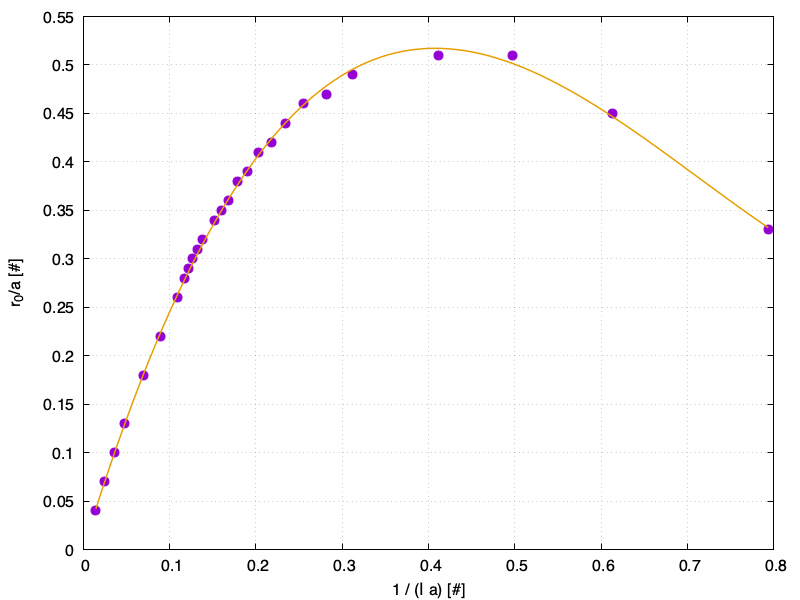
\includegraphics[width=0.9\textwidth]{Graf/effective_range.png}
%\caption{Effective range behaviour with respect to the cut-off $\lambda$. The parameters $\alpha$, $\beta$, and $\gamma$ in equation \ref{eq:philips_effr} are respectively 2.9, -5.0, and 2.4 . those number are of order $\sim 1$ as expected.}
%\label{fig:fig1}
%\end{center} 
%\end{figure}




%Is this necessary?
%\textbf{Few different scales can be identified in this study}.
%The mass of the fermions define the system we are studying, however, any physical observable can be rescaled according to it without changing the qualitative nature of the system.
%For compatibility with our numerical methods, the mass is taken to be the nucleon one, therefore; scattering lengths, effective radii, point-like radii will be measured in fm, and energies and cut-offs will be defined in MeV. 
%The mass of the degrees of freedom is also the only breaking scale of our toy theory since the study of long range interaction scale is not in the goals of this study. 
%However, extra attention is require in the case of nuclear interaction, where the pion mass scale is still relatively close to the typical momentum exchanged.
%The second scale is the scattering length, which, by definition, is much larger than the typical interaction range.
%However, interaction with infinite scattering length are difficult to be treated numerically, therefore, in this work we will use mainly large, but finite, $a_0$. 
%The scattering length is also proportional to the inverse of the two-body binding: $\sim \frac{1}{\sqrt{B_2}}$ \cite{PhysRev.76.18}, which should be much smaller than the breaking scale of the theory.
%The three-body binding breaks the universality of the systems.
%It defines the number and deepness of many-body bound states in the few- and many-body systems.
%In the case of three bosons or spatially symmetric fermions the energy ratio between such states is determined by Efimov physics \cite{Efimov:1970zz,Efimov:1973awb}.
%In this work the three-body LEC is chosen to create one and only one three-body bound state with energy $B_3$.
%In table \ref{tab:configurations} are listed the different configurations of two- and three-body bindings used in this work.
%Finally, the cut-off, or equivalently, the effective range of the two-body interaction (see equation \ref{eq:philips_effr}) can be also treated as a scale of the theory.
%Even if it is expected to be irrelevant since the cut-off should be taken to be large, theory artifacts can be studied in relation to the residual effective range magnitude.





\section{Results}


\begin{figure}
    \centering
    \begin{subfigure}[t]{0.45\textwidth}
        \centering
        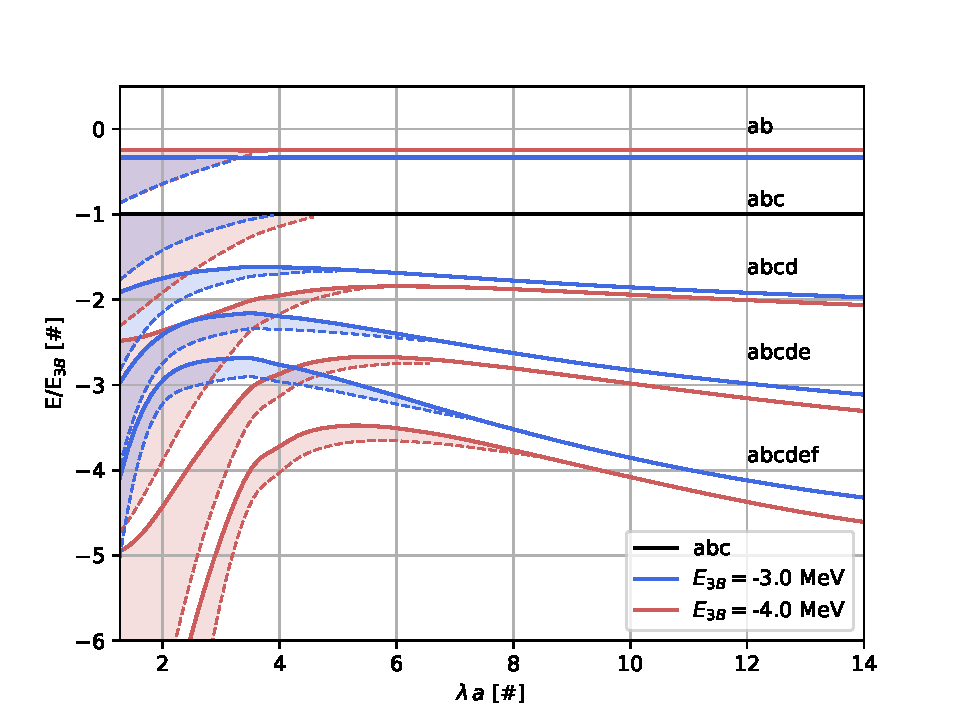
\includegraphics[width=\linewidth]{./p-systems-vs-l} 
        \caption{Colors online. Ground-state energy behaviour of $A$ (solid line) and $A+1$ (dashed line) $A-$flavours fermionic system with respect to the cut-off used. The blue line represent the theory fitted on the configuration A3 and the red represent the A4 one (see \tabref{tab:configurations} and text for the configuration specifics). }
        \label{fig:treshold}
    \end{subfigure}
    \hfill
    \begin{subfigure}[t]{0.45\textwidth}
        \centering
        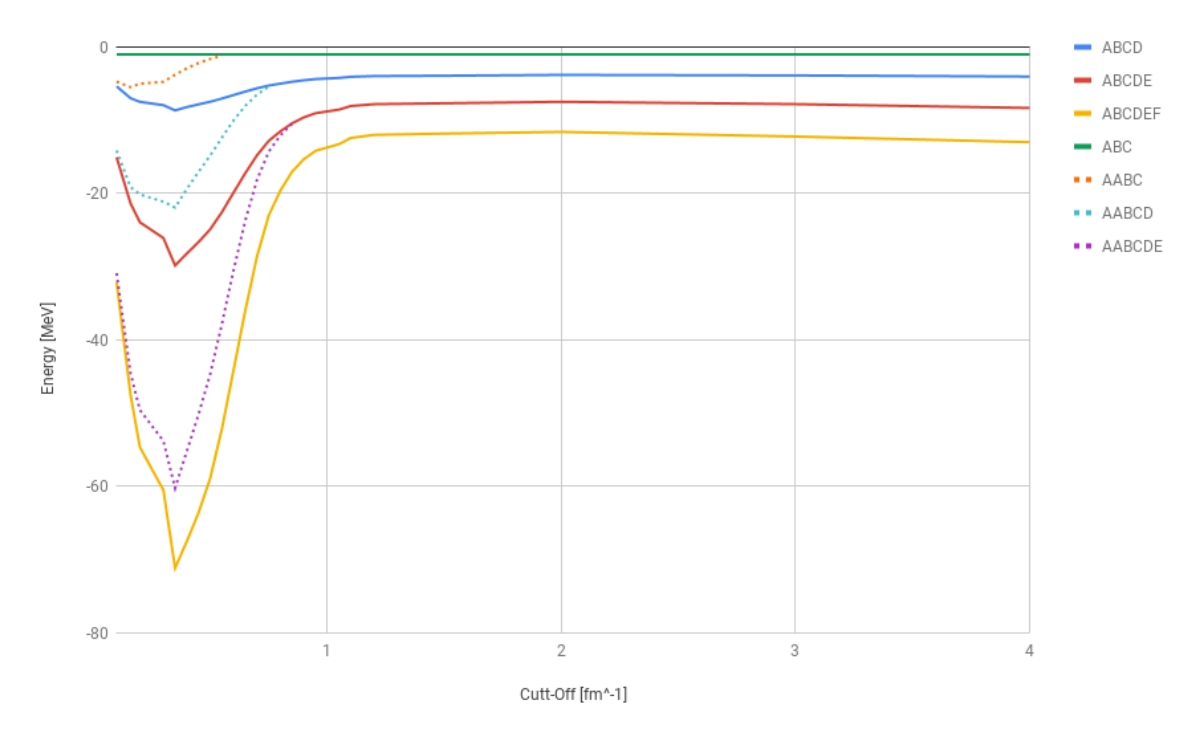
\includegraphics[width=\linewidth]{./unitarity_chart} 
        \caption{Ground-state energy behaviour of $A$ (solid line) and $A+1$ (dashed line) $A-$flavours fermionic system with respect to the cut-off used in the unitary limit. The two-body LEC is fitted to zero energy threshold, the three body LEC is fitted to reproduce a unique $B_3=4$ MeV three body bound state. See text for the figure description.}  
        \label{fig:unitary}
    \end{subfigure}
\caption{}
\end{figure} 

The $A$-boson ground states of a theory characterized by a Hamiltonian of
type \eqref{eq:hamiltonian}
has been numerically analysed in detail (see \eg~ \cite{Bazak:2016wxm,2015PhRvA..92c3626Y,Gattobigio:2012tk,vonStecher:2011zz,Gattobigio:2011ey}).
In contrast to these studies, the bosonic interaction of this work supports
exactly one bound dimer and one trimer. The universal accumulation of trimers
at the $1+1$ body threshold is not considered. Furthermore, for all considered
ratios $B(3)/B(2):=\Lambda^*$, only one $(A+1)$-boson state is found below
the $A$-boson threshold and no second as established numerically, \eg, in Refs.~
\cite{Hammer:2006ct,2009NatPh...5..417V,vonStecher:2011zz}.
Comparing the $A<7$ body spectra of $\Lambda^*=4$ with $\Lambda^*=3$ in
\figref{fig:treshold}, $B(A)/B(3)$ reduces, too. This indicates, that these states
resemble the shallow components of the conjectured universal pair. This hypothesis is
based on the argument that $\Lambda^*\to0$ is realized with an increasingly repulsive
three-body interaction which precludes the emergence of further $A$-boson bound states
but has an enhanced effect in a larger system as the number of triplets grows
with $A$. Therefore, one na\"ively expects a more rapid decrease of $B(A)$ \wrt $B(A-1)$ which compensates the initially found wider gap. To parametrize the
number $A^*$ at which $B(A^*+1)<B(A^*)$, \ie, stable $(A^*+1)$-body
cluster cease to exist, remains an open question.
For this work, we assume that $A^*=2$, which
means that for moving the trimer bound state closer to the dimer-boson threshold
the larger systems remain stable but they accumulate at the trimer-$(A-3)$-boson
threshold. This accumulation resembles the set of shallow states of the
alleged universal pair.

These considerations which identify the observed $A$-body states as ground
states are useful to characterize their spatial structure. The variational
bases expand only states with $L_\text{total}=0$. Yet, spatial configurations with
mixed symmetry are, in principle, allowed. However, interaction matrix elements
of such mixed states, \eg, particles occupying different oscillator $S$-shells
\scalebox{0.8}{$\young(\es,\zs)$}, 
should be of higher energy than a totally symmetric state
\scalebox{0.8}{$\young(\es\es)$}. For the three and four-body states we verified
this conjecture numerically i 

\noindent\rule{\textwidth}{1pt}

The states are spatially totally symmetric, they are bound with respect to the
$B(A-1)$ threshold, the convergence rate of $B(A)$ and $\rms{A}$ (within the considered cutoff range
$\Lambda\in[0.1,14]~\text{fm}^{-1}$) increases with $B(3)/B(2)$, \ie, closer to the 2-body unitarity limit, the bosonic
ground states become less sensitive with respect to details of the two- and three-body interactions.

Subsequently, one particle was added to these $A$-boson systems, not only with the same mass as the others, but also 
flavour-equal to one of them.
The identity of two of the $A+1\in[3,7]$ particles was enforced on the SVM basis states which where totally
antisymmetric with an $A$-dimensional internal space. For $2+1$ particles, \eg, the spin-up/down states of a neutron suffice,
while for $4+1$, the spin and isospin formalism can be invoked.

With this implementation of the statistical nature of the particles, the SVM evaluations yield $B(A+1)<0$, \ie, no bound 
states,
{\bf if} the spatial component of the variational basis states was constrained to
a total orbital angular momentum $L_\text{total}=0$.
Although, this can be proven analytically\footnote{} for contact interactions,
finite interaction ranges, \ie, $\forall\Lambda<\infty$, especially for $\Lambda\ll 1~\text{fm}^{-1}$, such 
bound states cannot be ruled out, {\it a priori} because: one, a state with $L_\text{total}=0$ has non-zero overlap with 
mixed-symmetry states (as they are enforced by the internal wave-function component), and two, the finite range allows for 
non-zero matrix elements of the interaction even if two particles reside in different orbitals.
However, the results demonstrate the smallness of such transitions for reasonable ranges,
which are necessary for the binding.

If the spatial component of the variational basis is projected onto $L_\text{total}=1$, the eigenvalue spectrum of
the $A+1\in[3,7]$ particle systems contains a negative value ($B(A+1)$; if not noted otherwise, this notation
implies $L_\text{total}=1$) for $\Lambda\approx0.1~\text{fm}^{-1}$.
In prose, if the regularized interaction provides enough attraction beyond a repulsive region in which an effective
angular momentum barrier drives the particles apart, the system's ground state is bound.
In order to assess the universal character of such a stable bound state with mixed symmetry -- is $B(A+1)$ correlated
with $B(2,3)\neq f(\Lambda)$ by renormalizing the coupling strengths in \eqref{eq:hamiltonian} -- the cutoff
is varied: $\Lambda\in[0.1,14]~\text{fm}^{-1}$.

With increasing cutoff, \ie, decreasing interaction range, \ie, approaching the contact limit, $B(A+1)$ is found to decrease
and vanish for some critical value $\Lambda_c$ which increases linearly with $A$ (see \figref{fig:RGM1}).
The more particles in the bosonic ground-state core, the shorter-ranged the microscopic two- and three-body interaction
has to be in order not to stabilize the $A+1$ mixed-symmetry state.
As $\Lambda_c(A=2-6)$ are arguably small relative to a scale above which the nuclear contact theory (\eftnopi) would
be useful, the result implies: the absence of $L=1$, $S=1/2$, $A+1$-body bound states in an $A$-flavour theory
is a consequence of flavour-independent contact interactions which are renormalized to one bound dimer and one trimer. 

Strictly speaking, the results presented thus far support this conclusion about the universal instability of the $A+1$
body state only for $A=2-6$. In order to gain insight whether the linear dependence of the critical range holds for
$A>6$, we employ a single-channel, effective two-fragments resonating-group approximation. This approximation
turns the $A+1$ body problem into a tow-body problem between a ``frozen'' core and one of the original particles of
the few-body problem. What makes this seemingly drastic simplification appropriate is the halo character of the problem,
namely, the increasingly large gap $\lim_{\Lambda\to\infty}\left[B(A)-B(A-1)\right]=\infty$, which does not
allow for excitations of the bosonic core induced by the $A+1$-th particle if the energy of the latter
does not exceed the scale set by this gap. It is helpful to consider this treatment as a generalization of the
time-honoured description of the 5-nucleon system around the Nucleon-$\alpha$ threshold.

However, the RGM method does not model the core as point-like but retains its finite. It assumes
an independent motion of the core particles but takes into account (anti)symmetrization.
The independent motion allows for a representation of the core by
its $A$-body ground state as it exists in the absence of the $A+1$-th particle.
As this state was shown
to be spherically symmetric with $L_\text{total}=0$, we choose to retain only one component of an harmonic-oscillator (HO)
Slater-determinant expansion, \ie, a product of four single-particle HO ground-state orbitals.
The $A+1$-body Schr\"odinger equation reduces to its 2-body form by disregarding variations of this wave function
while minimizing the corresponding functional only \wrt~the component which describes the relative motion.
In this course, the effect of the antisymmetrization between two of the particles has to be considered and is reflected
in isolated components of the effective 2-body potential.

We detail the parametrization of these various components of the core-particle interaction with the
microscopic coupling strengths $C_0$, $D_0$, the single-particle mass $m$, and the regulator parameter $\Lambda$
elsewhere. It is customary to present the effective potential as three term in the equation:
The direct potential, which averages the interaction of the orbiter with the core particles. This interaction is
local and resembles the character of the two-particle interaction for the fragment-relative coordinate. It does not
consider the statistical properties of the particles.
These properties lead to the non-local exchange interaction which contains an energy-dependent part which
is conventionally called the exchange kernel.

We shall discuss the case which disregards the exchange of the orbiter with one of the core constituents (local
approximation) before the results which employ the antisymmetrization \wrt~this pair in the RGM equation.
In both cases, the conjectures are presented before substantiating them with the data in \figref{fig:RGM}.

A non-relativistic system of $A+1$ particles with identical masses and
an $A$-dimensional internal flavour space cannot sustain a bound state if
its dynamics is constrained by representations of two- and three-particle
momentum-independent contact interactions which are renormalized to yield
a bound/unitary two-body state and a bound three-body state and whose
residual finite-range is below a critical value ($\lambda_c^{−1}$)
which decreases with increasing particle content $A$ of the system.
If the range of the regulated contact interactions, however, surpasses the
critical range, the ground state of the $A+1$ particles is bound with respect
to breakup in the bosonic, spatially symmetric $A$-body ground state and a
single free particle. The total orbital angular momentum of this $A+1$ bound
state is $L_{\text{\scriptsize total}}= 1$.
For any finite ratio $\Lambda^*<\infty$,
the critical range reaches a minimum at a certain number of particles $A$.


\newpage
Defining an effective theory as in equation \ref{eq:hamiltonian} with $C_0$ and $D_0$ fitted to reproduce the two- and 
three-body energies defined in \tabref{tab:configurations}, the energy of varius P-wave systems are calculated.
Using SVM the ground state energies of up to $A+1=$ 7 isomassive fermions with $A \le $6 flavors are calculated.
The same is done up to $A+1\sim$60 $A$-flavour fermionic systems using resonating group method (RGM).
In the case of $A$ \textit{different} fermions the ground state is spatially symmetric.
No spin dependence is included in our model, therefore, those systems behaves as if composed of bosons (it is boson-like) 
and are equivalent to the case discussed in \cite{manybosons}.
Convergence of the ground state energy of bosonic-like system with respect to the cut-off is observed for all the theory 
input used in this work.
We observe and increasing of the ground state binding with the number of particles. 
The point radius $\langle r^2 \rangle$ has been calculated for $A\le6$, for a number of systems too small to extrapolate the 
behavior for large $A$, however, we expect it to behave as $A^{1/3}$ as predicted by the neutron drop model and observed in  
\cite{manybosons}.

Adding an extra fermion with the same flavor as one in core to the system, we observe the groundstate wavefunction to be 
spatially asymmetric, and with angular momentum L=1.
However, this state remains stable only for small cut-off after which the systems breaks in the symmetric core and the extra 
fermion.
This is a common behaviour of all the systems and input configurations considered.
In \figref{fig:treshold}, are compared the ground-state energy of the $A\le 6$  bosonic-like fermionic system and the 
L=1 $A$+1 bindings for $B_3=3$ and $4$ MeV.
For each number of particles a critical cut-off $\Lambda_c^A$, corresponding to the cut-off in which the $A+1$ state becomes 
unstable, exists.
For larger cut-offs, the ground-state energy coincide with the one of the $A-$fermion systems and the system breaks in a $A-$
particles symmetric subsystem and a free fermion.
The result for $A^2B$ fermions is in agreement with the one found by Kartavtsev et al. \cite{Kartavtsev_2007} in the 
particular case in which the fermions are isomassive.

\begin{figure}
\centering
\begin{subfigure}[t]{0.49\textwidth}
\centering
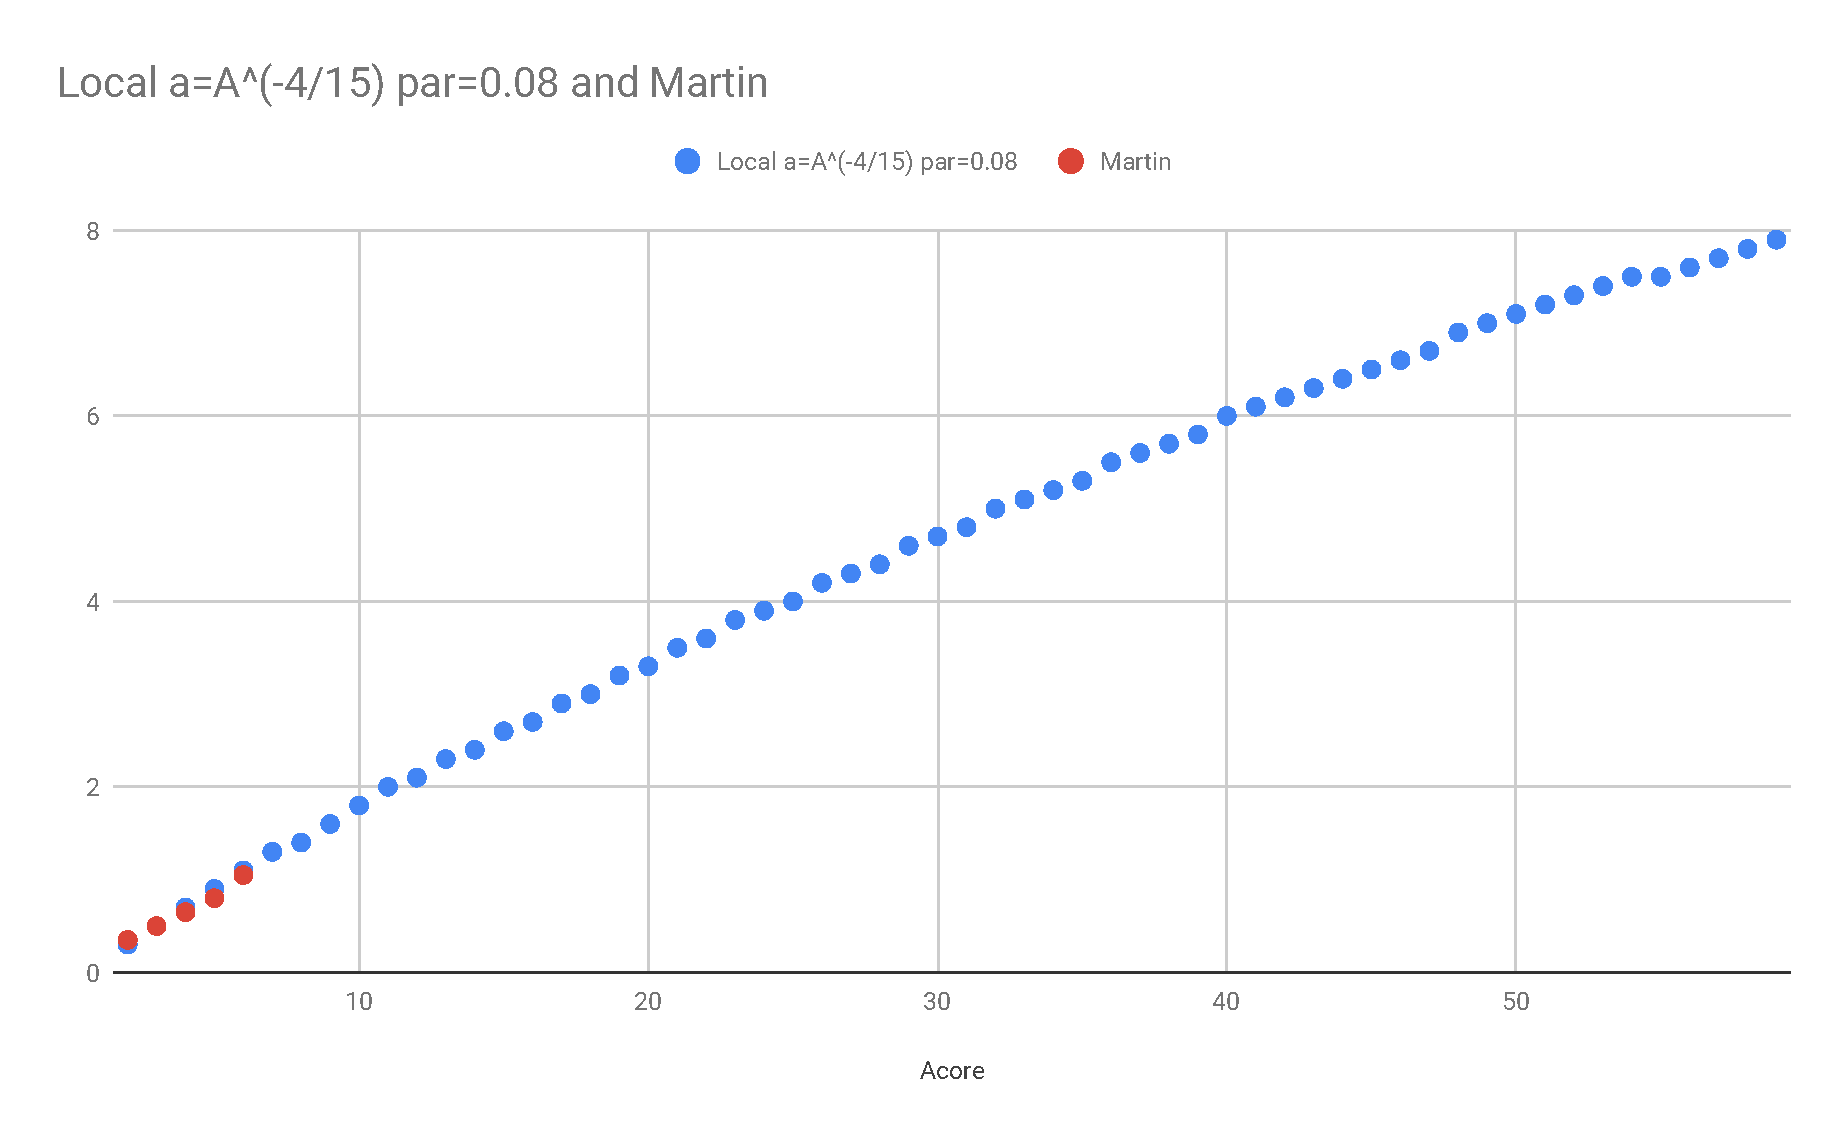
\includegraphics[width=0.9\textwidth]{./local2}
\caption{}
\label{fig:RGM1}
\end{subfigure}
    \hfill
\begin{subfigure}[t]{0.49\textwidth}
\centering
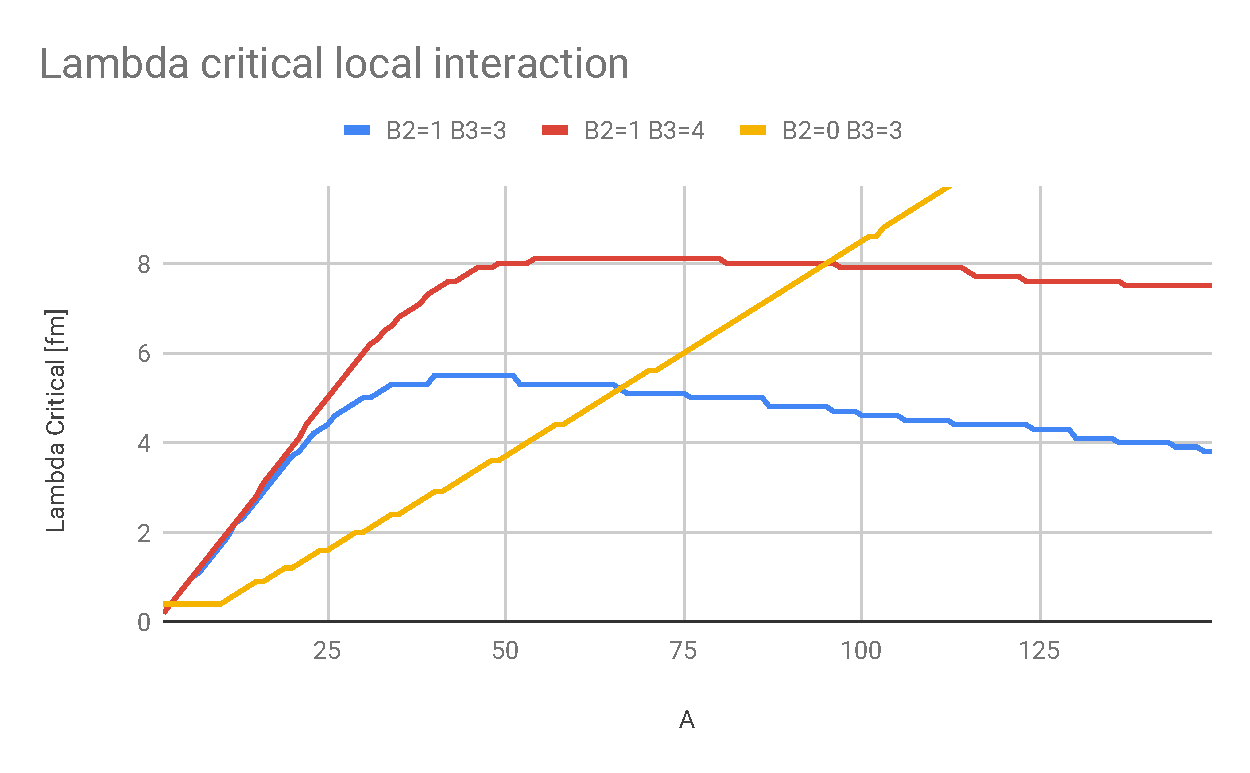
\includegraphics[width=0.9\textwidth]{./local_large} 
\caption{}        
\label{fig:RGM2}
\end{subfigure}
\caption{Dependence of the critical cutoff ($\lambda_c$) on the number of core particles ($A$).
Red dots in (a) mark SVM few-body calculations.
All other curves represent results obtained within a single-channel resonating-group method.
In (b), the effect of a change in the ratio between two- and three-boson binding energies on $\lambda_c$ is shown.
For $B(2)=0$, the respective scattering length $\to\infty$.}
\label{fig:RGM}
\end{figure}

\textbf{Larger systems} are not accessible with ab-initio few-body methods like SVM. 
For this purpose an extension of resonating group method (RGM) \cite{PhysRev.52.1083,Naidon_2016} has been developed.
From the fundamental two- and three-body interaction, a potential between the spatially symmetric core and the remaining fermion is extracted. 
In principle this permits to reduce a complex many-body calculation in a simpler two-body problem at the price of having non-local and energy dependent interaction.
The derivation is done assuming that the wave function of the core is frozen to be the harmonic oscillator (HO) Hartree Fock (HF) ground state with respect to the system center of mass.
The oscillator parameter is fixed to reproduce the HO ground state point radius $\sqrt{\langle r^2 \rangle} \propto A^{1/3}$.
$\alpha$ is fitted to reproduce the $\Lambda_c^{3\le A \le 6}$ from SVM calculations.
In \figref{fig:RGM} is shown the behavior for $A \le 60$ using RGM with local approximation for different configuration of the theory. 
We observe an increasing of $\Lambda_c^A$ with $A$, remaining finite for all the systems considered.
In one hand, this means that adding more particles in the spatially symmetric core of the system, the P-wave states becomes more stable and for any $r_0$ there is a minimal $A$ after which it stabilize (see equation \ref{eq:philips_effr} for $\Lambda\Leftrightarrow r_0$ correspondence).
On the other one, there is always a $\Lambda_c^A$ for which the P-wave state becomes unstable and in the contact limit all P-wave systems decay in the symmetric core and one particle.
Comparing  $\Lambda_c^A$  with the scale of the system (the mass of the particles), it results that the unstability always happens far from the expected renormalization invariant reagion.
This remains true also when we consider nuclear mesonic scales.
In facts, introducing a new breaking scale $M_{hi}\sim M_{\pi}\approx 140$ MeV we expect to reach renormalization invariance for $\Lambda\ll M_{\pi} a \sim 10-40$ which is larger or comparable with the critical cut-off we observe.

--- This behavior can be seen for different configuration of two and three body bindings close to universality.
Studying $\Lambda_c^A$ behavior with the non-universal parameter $B_3/B_2$ ... need more data here to do the comparison. ---


\begin{figure}[h] 
\centering 
\begin{floatrow}
\ffigbox{
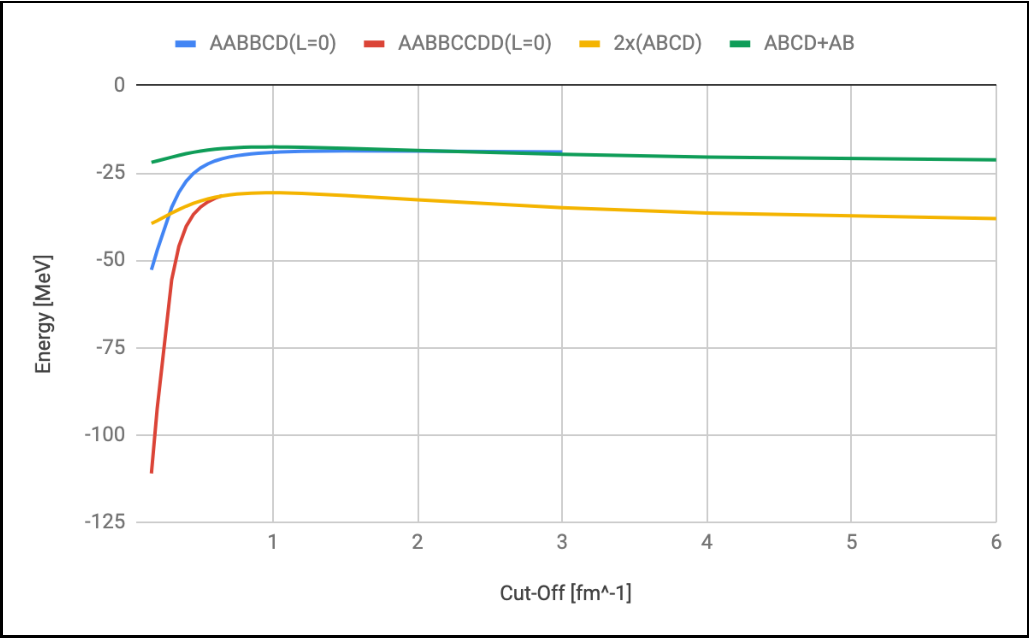
\includegraphics[width=0.45\textwidth]{./Nuclear} 
}{
\caption{Energy of $^8$Be, $^6$Li and the relative thresholds with respect the cut-off. The instability of P-wave system is observed also if the theory is fitted to reproduce nuclear two- and three-body bindings.}
\label{fig:nuclear}
}

\capbtabbox{%
\centering 
\begin{tabular}{ccc}
System & $(AB)^2$ & $(AB)^2CD$ \\\hline\hline
Total L & $r_c$ [fm]& $r_c$ [fm]\\
0 & 4.16 & 1.23 \\
1 & 5.21 & 2.96 \\
2 & 4.81 & 2.30 \\
\end{tabular}
}{\caption{Minimum effective range that stabilize the 2+2 (two dimers) and the 4+2 (analugus to $^6Li$ in nuclear physics) for different partial waves. Despite the simple interaction the level order well represent the one observed for $^6Li$ \cite{Chadwick20112887}. Nonetheless, for small effective range (large cut-off) all these states become unstable. }\label{tab:levelorder}}
\end{floatrow}
\end{figure} 


\textbf{The nuclear case} is studied fitting the two-body energy to the deuterium binding $B_2=2.22$ MeV and $B_3$ to the $B(^3He)=8.48$ MeV ground state. 
No spin dependence is included in the interaction, therefore, spin singlet dibaryon (e.g. the dineutron) results as bound as the deuterium.
However, nuclear physics do not hardly break spin symmetry and we expect our result to be qualitatively accurate.
We observe the same instability pattern shown in \figref{fig:treshold} for all the A+1 systems with $A\le 4$.
However, in the nuclear case, none of these systems are expected to be stable. 
More interesting is $^6$Li, which is expected to have a stable bound-state with L=1.
Our calculations show (see \figref{fig:nuclear}) that this state stability is supported only for a limited range of cut-off and the system breaks in a deuterium and an alpha particle.
The calculation for $^8$Be leads to similar results and an instability with respect to alpha decay.
Studying the spectrum of the $A^2B^2CD$ system ($^6$Li if fitted on nuclear observable), more than one state appear to be stable for very small $\Lambda$.
All those states becomes unstable for large $\Lambda$. 
Studying the order of the states and the order of disappearance (see \tabref{tab:levelorder}), it well represent the expected one for the physical $^6$Li despite the oversimplified interaction used.

Inspecting the scale of the critical cut-off with respect to the other present in the theory it can be argued that $\Lambda_c$ for $^6$Li is of the same order  as the pionmass breaking scale $\Lambda_c\sim1.5$ fm$^{-1} \approx300$ MeV.
In EFT the cut-off of the theory should be pushed to be much larger that the expected breaking scale in order to be able to define the powercounting.
Therfore, we conclude that the presence of a stable six-body bound state is a cut-off artifact.
Nonetheless, a less puristic approach of the theory whit a finite range interaction might be still able to bind the six-body system. 
This methodology might be successful to describe small and even medium-large nuclei, but it mixes different orders of the powercounting making hard to have a consistent estimation of theoretical uncertainties.


\begin{figure}[h] 
\centering 
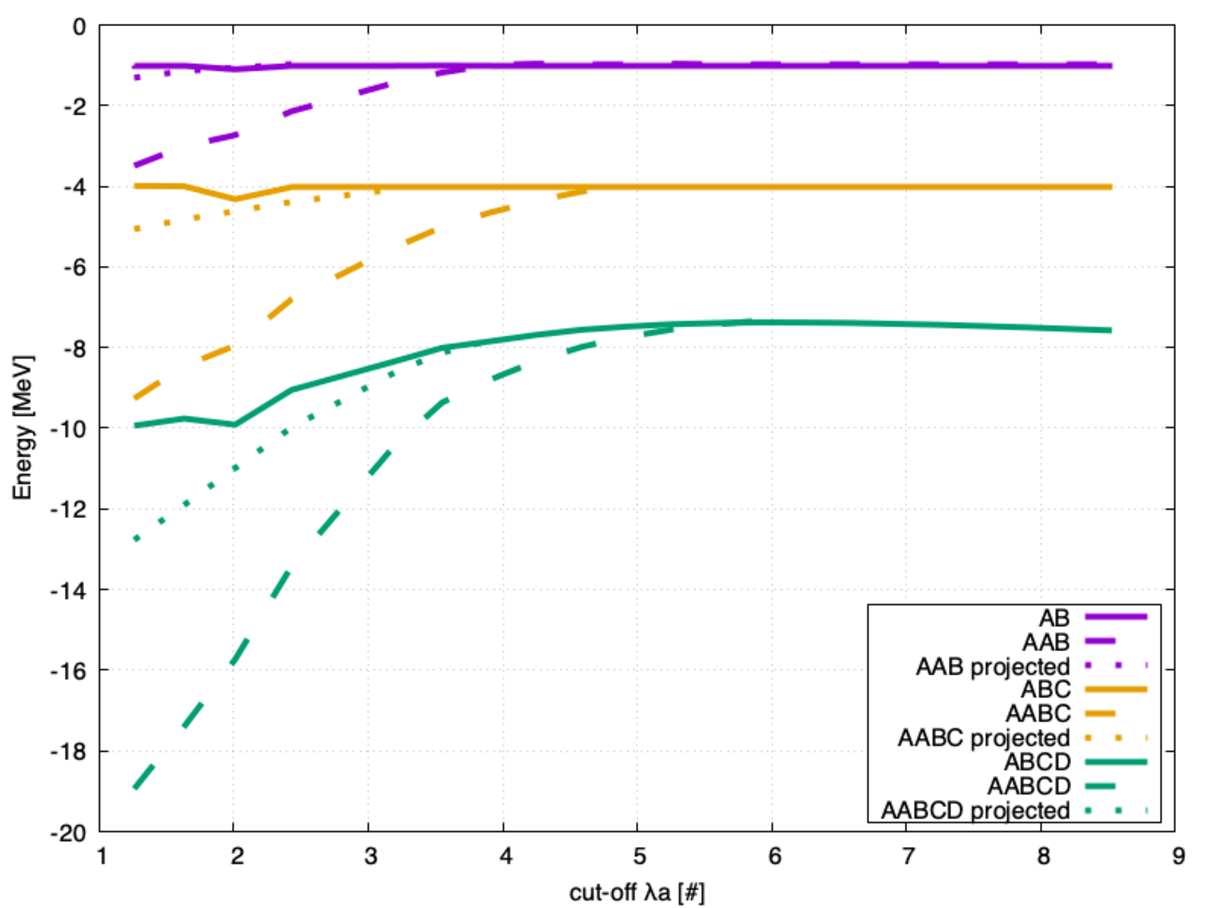
\includegraphics[width=0.8\textwidth]{./Sprojection} 
\caption{Energy of the A+1 fermionic systems with projected (dotted line) and not projected (dashed lines) compared witht the energy of the bosonic like core with A spatially symmetric fermions.}
\label{fig:Sprojection}
\end{figure} 

\textbf{Projecting the interaction} discriminate between the contribution of different partial waves ( and different orders of the theory) included into the finite cut-off interaction.
In facts, the Gaussian regulator expanded in partial waves contains any-order partial waves.
Larger angular momentum contributions disappear only when the cut-off is increased, but are still relevant in the region in which P-wave states are stable. 
In other words, finite range interaction does not only describe a finite and large S-wave scattering length but is also contaminated by finite larger-order ERE parameters in S-wave, as the S-wave effective range and the scattering volume for L=1.
Both this contributions are expected to enter only subleading in the system description but contribute to the stabilization of P-wave systems at low cut-off.
To study which partial waves mostly contribute to the system binding we project the four-flavor system in asymmetric spinorial state.
This forces the spatial part to be symmetrical, (even total angular momentum). 
We observe a great reduction of $\Lambda_c^A$ (shown in \figref{fig:Sprojection}) which indicates that residual odd angular momentums play a fundamental role in the system stability.
The residual binding is due to S-wave effective range and large even angular momentum (L=2) contributions.
This observation does not prove that a P-wave interaction will stabilize P-wave states above $\Lambda_c^A$, but suggests that it might help to extend contact EFT to multi-fermionic systems.

\textbf{The pole movement} with respect to $\Lambda$ when the system becomes unstable is another important aspect of this study.



\section{Discussion and conclusions}

\newpage
\section*{References}
\bibliographystyle{ieeetr}
\bibliography{Thebibliography.bib}
\end{document}
